\section{Two-phase flow with phase appearance and disappearance}
\subsection{}
\begin{frame}
\frametitle{Two-phase flow with phase appearance and disappearance}
\vspace*{-0.6 cm}
\begin{equation*}
\dps
\left\lbrace\begin{array}{llccc}
\dps \partial_t l_\componentw(\textcolor{cadmiumgreen}{\Sl}) + \nab \cdot {\bm \Phi}_{\mathrm{w}}(\textcolor{cadmiumgreen}{\Sl,\Pl,\chihl}) = Q_{\componentw}, \\
\dps \partial_t l_\componenth(\textcolor{cadmiumgreen}{\Sl,\Pl,\chihl})  + \nab \cdot {\bm \Phi}_{\mathrm{h}}(\textcolor{cadmiumgreen}{\Sl,\Pl,\chihl})=\Qh,\\
\textcolor{electricpurple}{1 - \Sl} \geq 0, \;  \textcolor{carmine}{H\left[\Pl + \Pcp(\Sl) \right] - \beta_{\phasel} \chihl} \geq 0, \; \left[\textcolor{electricpurple}{1 - \Sl} \right] \cdot \left[\textcolor{carmine}{H\left[\Pl + \Pcp(\Sl) \right] - \beta_{\phasel} \chihl}\right]=0  
\end{array}
\right.
\end{equation*}
\vspace{0.3 cm}
\invisible<1>{
\hspace*{-0.15 cm} \textcolor{midnightblue}{\textbf{Unknowns:}} liquid saturation $\textcolor{cadmiumgreen}{\Sl}$, liquid pressure $\textcolor{cadmiumgreen}{\Pl}$, mole fraction of liquid hydrogen $\textcolor{cadmiumgreen}{\chihl}$ \\
\vspace{0.3 cm}
\invisible<2>{
\textcolor{midnightblue}{\textbf{Linear functions:}} amount of water $l_\componentw$, amount of hydrogen $l_\componenth$\\
\vspace{0.3 cm}
\invisible<3>{
\textcolor{midnightblue}{\textbf{Nonlinear function:}} capillary pressure $\Pcp$ \\
\vspace{0.3 cm}
\invisible<4>{
\textcolor{midnightblue}{\textbf{Nonlinear fluxes:}} water flux $\underbrace{{\bm \Phi}_{\mathrm{w}}}_{\mathrm{Darcy} + \mathrm{Fick}}$, hydrogen flux $\underbrace{{\bm \Phi}_{\mathrm{h}}}_{\mathrm{Darcy} + \mathrm{Fick}}$\\
\vspace{0.3 cm}
\invisible<5>{
\textcolor{midnightblue}{\textbf{Nonlinear complementarity constraints:}} $\Rightarrow$ \textbf{Phase change}\\
\vspace{0.2 cm}
\scriptsize{Ben Gharbia and Jaffré (2014)}

\invisible<6>{
}}}}}}

\end{frame}
%

%
%% DISCRETIZATION FINITE VOLUME
% \begin{frame}
% \frametitle{Discretization by the finite volume method}
% \textcolor{blue}{\textbf{Numerical solution: }}
% \begin{equation*}
% \bUn \egaldef (\bUn_K)_{K\in \Th}, \qquad \bUn_K \egaldef  (\SKn,\PKn,\chiKn) \quad \textcolor{cadmiumgreen}{\textbf{one value per cell and time step}} 
% \label{eq:finite:volume:approx}
% \end{equation*}
% \textcolor{cadmiumgreen}{\textbf{Time discretization:}}
% \\
%  \begin{figure}[htbp]
% \vspace{-0.6 cm}
%  \centering
%  \begin{picture}(200,60)(0,0)
%  \thicklines
%  \put(0,15){\line(200,0){200}}
%  %\put(0,10){\red{\line(0,10){10}}}
%  \put(0,0){\makebox(0,0){\small \red{$t_0 = 0$}}}
%  \put(0,15){\black{\circle*{6}}}
%  \put(25,10){\red{\line(0,10){10}}}
%  \put(25,0){\makebox(0,0){\small \red{$t_1$}}}
%  %\put(25,15){\blue{\circle*{6}}}
%  \put(12.5,30){\makebox(0,0){\small  \blue{$I_1$}}}
%  \put(50,10){\red{\line(0,10){10}}}
%  \put(50,0){\makebox(0,0){\small \red{$t_2$}}}
%  %\put(75,15){\blue{\circle*{6}}}
%  \put(37.5,30){\makebox(0,0){\small  \blue{$I_2$}}}
%  \put(75,30){\makebox(0,0){\small \blue{$\cdots$}}}
%  \put(75,0){\makebox(0,0){\small \red{$\cdots$}}}
%  \put(112.5,30){\makebox(0,0){\small \blue{$I_{n}$}}}
%  %\put(215,15){\blue{\circle*{6}}}
%  \put(100,10){\red{\line(0,10){10}}}
%  \put(100,0){\makebox(0,0){\red{\small $t_{n-1}$}}}
%  \put(125,10){\red{\line(0,10){10}}}
%  \put(125,0){\makebox(0,0){\red{\small $t_{n}$}}}
%  \put(150,30){\makebox(0,0){\small \blue{$\cdots$}}}
%  \put(150,0){\makebox(0,0){\small \red{$\cdots$}}}
%  \put(175,0){\makebox(0,0){\small \red{$t_{\Nt - 1}$}}}
%  \put(175,10){\red{\line(0,10){10}}}
%  %\put(355,15){\blue{\circle*{6}}}
%  \put(187.5,30){\makebox(0,0){\small \blue{$I_{\Nt}$}}}
%  \put(200,0){\makebox(0,0){\small \red{$t_{\Nt} = t_{\mathrm{F}}$}}}
%  %\put(240,10){\red{\line(0,10){10}}}
%  \put(200,15){\black{\circle*{6}}}
%  \end{picture}
% \qquad \qquad
% 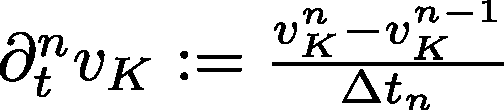
\includegraphics[scale = 0.5]{fig_article_chap_2/approx_time_derivative.pdf}
%  \end{figure}
% \begin{minipage}[c]{0.3 \textwidth}
% \textcolor{cadmiumgreen}{\textbf{Space discretization:}} $\Th$ a superadmissible family of conforming simplicial meshes of $\Omega$. \textcolor{blue}{Number of cells : $\Nsp$}
% \begin{equation*}
% \dps 
% \left(\nab v \cdot \bn_{K,\sigma},1\right)_{\sigma} := \dps |\sigma| \frac{v_L - v_K}{d_{KL}} \hspace{0.2 cm} \sigma = \overline{K} \cap \overline{L},
% \end{equation*}
% \end{minipage}
% \hfill
% \begin{minipage}[c]{0.5 \textwidth}
% \begin{figure}
% 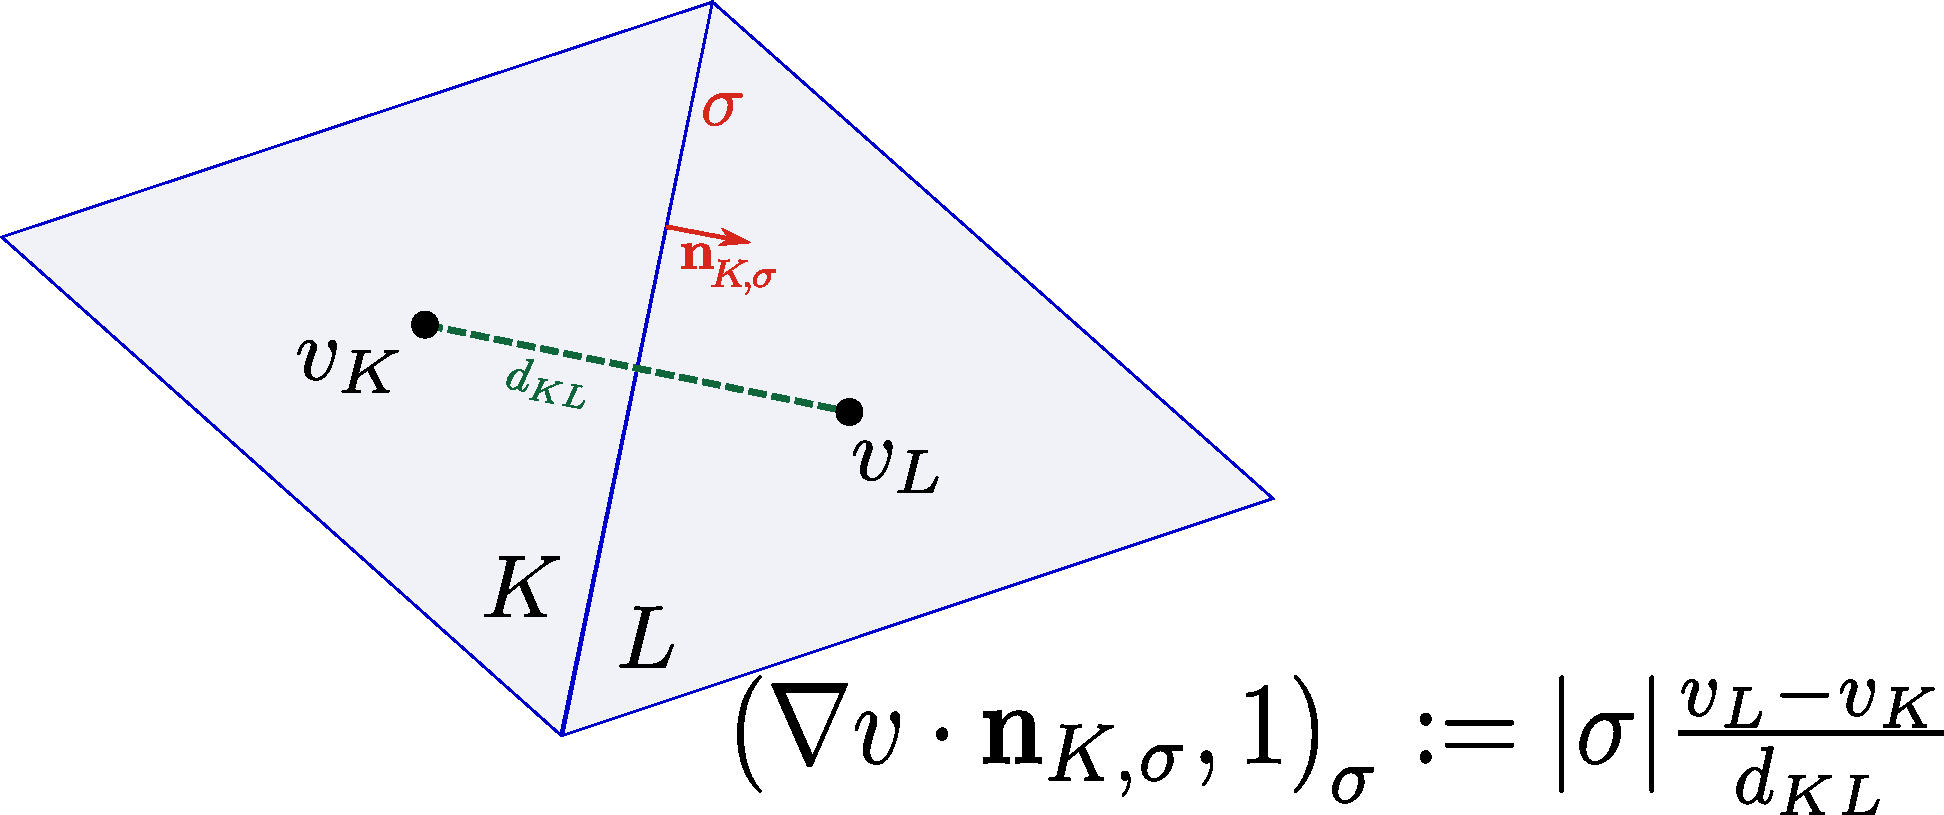
\includegraphics[width = 0.7 \textwidth]{fig_article_chap_3/gradient_discretization.pdf}
% \end{figure}
% \end{minipage}
% \end{frame}

\begin{frame}
\frametitle{Discretization by the finite volume method}
\textcolor{cadmiumgreen}{\textbf{Numerical solution: }}
\begin{equation*}
 \bUn \egaldef (\bUn_K)_{K\in \Th}, \qquad \bUn_K \egaldef  (\SKn,\PKn,\chiKn) \quad \textcolor{cadmiumgreen}{\textbf{one value per cell and time step}} 
\end{equation*}
\textcolor{blue}{\textbf{Discretization of the water equation}}
\begin{equation*}
S_{\mathrm{w},K}^n(\bU^n) \egaldef |K| \partial_t^n \lwK  + \sum_{\sigma \in \EK} {F}_{\componentw,K,\sigma}(\bU^{n})- |K|\QwKn = 0,
\end{equation*}
% \begin{equation*}
% {F}_{\componentw,K,\sigma}(\bUn) \egaldef \rhowl (\mobilityliq)_{\sigma}^{n} (\psil)_{\sigma}^{n} - (\jhl)_{\sigma}^{n} \quad \sigma \in \EKint \quad \overline{\sigma} = \overline{K} \cap \overline{L}.
% \end{equation*}
\invisible<1>{
\textcolor{blue}{\textbf{Discretization of the hydrogen equation}}
\begin{equation*} 
S_{\mathrm{h},K}^{n}(\bU^n)\egaldef |K| \partial_t^n \lhK + \sum_{\sigma \in \EK} {F}_{\componenth,K,\sigma}(\bUn) - |K| \QhKn = 0,
\end{equation*}
% \begin{equation*}
%  {F}_{\componenth,K,\sigma}(\bUn) \egaldef \betal \chisigman (\mobilityliq)_{\sigma}^{n} (\psil)_{\sigma}^{n} + (\psig)_{\sigma}^{n} (\mobilitygas)_{\sigma}^{n} (\rhog)_{\sigma}^{n} + (\jhl)_{\sigma}^{n} , \quad \sigma \in \EKint \quad \overline{\sigma} = \overline{K} \cap \overline{L}.
% \end{equation*}
\invisible<2>{
At each time step $t^n$, we obtain the nonlinear system of algebraic equations
\begin{equation*}
S_{c,K}^n(\bU^n)=0 \quad \forall K \in \Th \ \ \forall \componentc \in \left\{\componentw,\componenth\right\}
\end{equation*}
\invisible<3>{
}}}
\end{frame}
%
\begin{frame}
\frametitle{Discrete complementarity problem and semismoothness}
\textcolor{red}{\textbf{Discretization of the nonlinear complementarity constraints}}
\begin{equation*}
\textcolor{electricpurple}{\mathcal{K}(\bU_K^n)} \egaldef \textcolor{electricpurple}{1-\SKn} \quad \textcolor{carmine} {\mathcal{G}(\bU_K^n)} \egaldef  \textcolor{carmine}{H(\PKn\hspace{-0.05 cm}+\hspace{-0.05 cm}\Pcp(\SKn))-\betal \chiKn}
\end{equation*}
\pause
The discretization reads
\begin{equation*}
\begin{split}
&S_{c,K}^n(\bU^n)=0 \quad \forall K \in \Th \quad \forall \componentc \in \left\{\componentw,\componenth \right\}\\
& \textcolor{electricpurple}{\mathcal{K}(\bU_K^n)} \geq 0, \quad   \textcolor{carmine} {\mathcal{G}(\bU_K^n)} \geq 0, \quad \textcolor{electricpurple}{\mathcal{K}(\bU_K^n)} \cdot \textcolor{carmine} {\mathcal{G}(\bU_K^n)}=0 \quad \forall K \in \Th
\end{split}
\end{equation*}
\pause
\begin{itemize}
\item
\textcolor{cadmiumgreen}{\textbf{We reformulate the complementarity constraints with C-functions}}
\item
\textcolor{cadmiumgreen}{\textbf{We employ inexact semismooth linearization}}
\item
\textcolor{cadmiumgreen}{\textbf{Can we estimate the error?}}
\item
\textcolor{cadmiumgreen}{\textbf{Can we distinguish the error components?}}
\end{itemize}
\end{frame} 
%
\begin{frame}[noframenumbering]
\centering
\Huge{\textcolor{carmine}{A posteriori error estimates}}
\end{frame}
%%
\begin{frame}
\frametitle{Weak solution}
\begin{equation*}
X \egaldef L^2((0,\tF);H^1(\Omega)), \ Y  \egaldef H^1((0,\tF);L^2(\Omega)), 
%\ \widehat{Y} \egaldef H^1((0,\tF);L^{\infty}(\Omega)),\\
 \  Z \egaldef L_{+}^2((0,\tF);L^{\infty}(\Omega)) 
% \\ & \left\| \varphi \right\|_{X_n} \egaldef \int_{\In} \sum_{K \in \Th} \left(\varepsilon h_K^{-2} \left\|\varphi\right\|_K^2 + \left\|\nab \varphi\right\|_K^2\right) (t) \mathrm{dt}
\end{equation*}
\\
\vspace{0.5 cm}
\textcolor{blue}{\textbf{Assumption: There exists a unique weak solution satisfying}}
\begin{itemize}
\item
% $\Sl \in \widehat{Y}$, \ 
$\textcolor{electricpurple}{1-\Sl} \in Z$, \ $\lc \in Y$, \ $\Pl \in X$, \ $\chihl \in X$, \ $\Phic \in L^2((0,\tF); \HdivOmeg)$
\item 
$\dps \int_{0}^{\tF} \left(\partial_t \lc, \varphi \right)_{\Omega}(t)\,\mathrm{dt}-\hspace{-0.1 cm}\int_{0}^{\tF} \left(\Phic, \nab \varphi \right)_{\Omega}(t)\,\mathrm{dt} = \hspace{-0.1 cm} \int_{0}^{\tF} \left(\Qc, \varphi \right)_{\Omega}(t)\,\mathrm{dt} \quad \forall \varphi \in X$
\item 
$\dps \int_{0}^{\tF} \left(\lambda - \left(\textcolor{electricpurple}{1 - \Sl}\right), \textcolor{carmine}{H[\Pl+\Pcp(\Sl)]-\betal \chihl}  \right)_{\Omega}(t)\,\mathrm{dt} \geq 0 \quad \forall \lambda \in Z$
\item
the initial condition  holds
\end{itemize}
\end{frame}
% %

\begin{frame}
\frametitle{Error measure}
\vspace{-0.3 cm}
\begin{enumerate}
\item<1> 
\textcolor{cadmiumgreen}{\textbf{Dual norm of the residual for the components}}
 \begin{equation*}
\left\|\mathcal{R}_{\componentc}(\Shtaunki,\Phtaunki,\chihtaunki) \right\|_{\Xn'} \egaldef \sup_{\substack{\varphi \in \Xn \\ \left\|\varphi\right\|_{\Xn} = 1}}  \int_{\In} 
 \left(\Qc - \partial_t \lchtaunki , \varphi\right)_{\Omega}(t) + \left(\Phichtaunki,\nab \varphi \right)_{\Omega}(t)\,\mathrm{dt} 
 \end{equation*}
\pause
\item<2>
\textcolor{cadmiumgreen}{\textbf{Residual for the constraints}}
\begin{equation*}
  \mathcal{R}_{\mathrm{e}}(\Shtaunki,\Phtaunki,\chihtaunki) \egaldef \int_{\In}\left(\textcolor{electricpurple}{1 - \Shtaunki}, \textcolor{carmine}{H \left[\Phtaunki + \Pcp(\Shtaunki)\right] - \betal \chihtaunki} \right)_{\Omega}(t)\,\mathrm{dt}
\end{equation*}
\pause
\item<3>
\textcolor{cadmiumgreen}{\textbf{Error measure for the nonconformity of the pressure}} $\mathcal{N}_{p}(\Phtaunki)$
\pause
\item<4>
\textcolor{cadmiumgreen}{\textbf{Error measure for nonconformity of the molar fraction}} $\mathcal{N}_{\chi}(\chihtaunki)$
\end{enumerate}
\vspace{0.3 cm}
\begin{equation*}
\mathcal{N}^{n,\kk,\ii}  \egaldef \left\{\sum_{\componentc \in\mathcal{C}} \left\|\mathcal{R}_{\componentc}(\Shtaunki,\Phtaunki,\chihtaunki) \right\|_{X_n'}^2 \right\}^{\frac{1}{2}} + \left\{\sum_{\phasep \in \mathcal{P}}\mathcal{N}_{\phasep}^2 + \mathcal{N}_{\chi}^2\right\}^{\frac{1}{2}} + \mathcal{R}_{\mathrm{e}}(\Shtaunki,\Phtaunki,\chihtaunki)
\end{equation*}
\end{frame}
\begin{frame}
\frametitle{A posteriori error estimate distinguishing the error components}


\begin{theorem}
\begin{equation*}
\mathcal{N}^{n,\kk,\ii} \leq \etadiscnki + \etalinnki + \etaalgnki
\end{equation*}
\end{theorem}
\textcolor{red}{Construction of the estimators:} 
\begin{itemize}
\item Equilibrated component flux reconstruction in $\HdivOmeg$
\item Potential reconstruction in $H^1(\Omega)$ 
\end{itemize}
\end{frame}
%
% \begin{frame}
% \frametitle{Component flux reconstructions}
% \vspace{-0.1 cm}
% \textcolor{cadmiumgreen}{\textbf{The finite volume scheme provides}}
% \begin{equation*} 
%   |K| \partial_t^n \lcK + \sum_{\sigma \in \EK} {F}_{\componentc,K,\sigma}(\bUn) =  |K|\QcKn
% \end{equation*}
% \invisible<1>{
% \vspace{-0.1 cm}
% \textcolor{cadmiumgreen}{\textbf{Inexact semismooth linearization}}

% \begin{equation*}
% \label{eq:flux:equation}
%  \frac{|K|}{\Delta t}\left[\lcK\left(\bU^{n,\kk-1}\right) - \lcK^{n-1} + \mathcal{L}_{\componentc,K}^{n,\kk,\ii}\right] + \sum_{\sigma \in \EKint} \mathcal{F}_{\componentc,K,\sigma}^{n,\kk,\ii}- |K|\QcKn + {\bR}_{\componentc,K}^{n,\kk,\ii} = 0
% \end{equation*}
% \vspace{-0.1 cm}
% \invisible<2>{
%  \textcolor{blue}{Linear perturbation in the accumulation}
% \begin{equation*}
% \mathcal{L}_{\componentc,K}^{n,\kk,\ii} \egaldef \sum_{K' \in \Th} \frac{|K|}{\Delta t}  \frac{\partial \lcK^n}{\partial \bU_{K'}^n}(\bU_{K'}^{n,\kk-1}) \left[\bU_{K'}^{n,\kk,\ii}-\bU_{K'}^{n,\kk-1} \right]
% \end{equation*}
% \textcolor{blue}{Linearized component flux}
% \begin{equation*}
% \label{eq:linearized:semi:smooth:component:flux}
% \mathcal{F}_{\componentc,K,\sigma}^{n,\kk,\ii} \egaldef \sum_{K' \in \Th} \frac{\partial {F}_{\componentc,K,\sigma}}{\partial \bU_{K'}^n} \left(\bU^{n,\kk-1}\right) \left[\bU_{K'}^{n,\kk,\ii} -\bU_{K'}^{n,\kk-1} \right] + {F}_{\componentc,K,\sigma}\left(\bU^{n,\kk-1}\right)
% \end{equation*}
% \invisible<3>{
% }}}
% \end{frame}
% % 
%  \begin{frame}
%  \textcolor{cadmiumgreen}{\textbf{Discretization error flux reconstruction:}}
% \begin{equation*}
% \Thetachdiscnki|_{K} \in \RTzero(K) \quad \left(\Thetachdiscnki \cdot \bn_K,1 \right)_{\sigma} \egaldef F_{\componentc,K,\sigma}\left(\bU^{n,\kk, \ii}\right) \quad \forall K \in \Th
% \end{equation*}
% \invisible<1>{
%  \textcolor{cadmiumgreen}{\textbf{Linearization error flux reconstruction:}}
% \begin{equation*}
% \Thetachlinnki|_{K} \in \RTzero(K) \quad \left(\Thetachlinnki \cdot \bn_K,1 \right)_{\sigma} \egaldef \mathcal{F}_{\componentc,K,\sigma}^{n,\kk,\ii} -  F_{\componentc,K,\sigma}\left(\bU^{n,\kk, \ii}\right) \quad \forall K \in \Th
% \end{equation*}
% \invisible<2>{
% \textcolor{cadmiumgreen}{\textbf{Algebraic error flux reconstruction:}}
% \begin{equation*}
% \Thetachalgnkinu  \egaldef {\bm \Theta}_{\componentc,h,\mathrm{disc}}^{n,\kk,\ii+\nuu} + {\bm \Theta}_{\componentc,h,\mathrm{lin}}^{n,\kk,\ii+\nuu} - \left(\Thetachdiscnki + \Thetachlinnki \right)
%  \quad \forall K \in \Th
% \end{equation*}
% \invisible<3>{
%  \textcolor{red}{\textbf{Total flux reconstruction:}} 
% \begin{equation*}
% \Thetachnkinu \egaldef \Thetachdiscnki+\Thetachlinnki+\Thetachalgnkinu \ \textcolor{red}{\bm \in} \ \HdivOmeg
%  \end{equation*}
% \invisible<4>{
% }}}}
%  \end{frame}
% %
% \begin{frame}
% \frametitle{Error estimators}
% \textcolor{red}{Violation of physical properties of the approximate solution}
% \begin{equation*}
% \partial_t \lc + \nab \cdot \Thetachnkinu \neq \Qc \quad \Thetachnkinu \neq \Phichtaunki(t^n)
% \end{equation*}
% \textcolor{red}{Violation of the complementarity constraints}
% \begin{equation*}
% \textcolor{electricpurple}{1 - \Shtaunki} \ngeq 0 \quad \textcolor{carmine}{H\left[\Phtaunki + \Pcp\left(\Shtaunki\right)\right]-\betal \chihtaunki} \ngeq 0
% \end{equation*}
% \textcolor{red}{Nonconformity of the approximate solution}
% \begin{equation*}
% \Phtaunki \notin X \quad \chihtaunki \notin X
% \end{equation*}
% \pause
% \begin{enumerate}
% \item 
% \textcolor{cadmiumgreen}{\textbf{Discretization estimator}}
% \item
% \textcolor{cadmiumgreen}{\textbf{Linearization estimator}}
% \item
% \textcolor{cadmiumgreen}{\textbf{Algebraic estimator}}
% \end{enumerate}
% \end{frame}
%
\begin{frame}[noframenumbering]
\centering
\Huge{\textcolor{carmine}{Numerical experiments}}
\end{frame}
% 
\begin{frame}
\frametitle{Numerical experiments}
$\Omega$:  one-dimensional core with length $L = 200 m$. 
\\
\vspace{0.2 cm}
\textbf{Semismooth solver:} Newton-min
\\
\vspace{0.2 cm}
\textbf{Iterative algebraic solver:} GMRES.
\\
\vspace{0.2 cm}
\textbf{Time step:} $\Delta t = 5000$ years, 
\\
\vspace{0.2 cm}
\textbf{Number of cells:} $\Nsp = 1000$, \\
\vspace{0.2 cm}
\textbf{Final simulation time:} $\tF = 5 \times 10^{5}$ years.
\\
\vspace{0.2 cm}
\begin{figure}
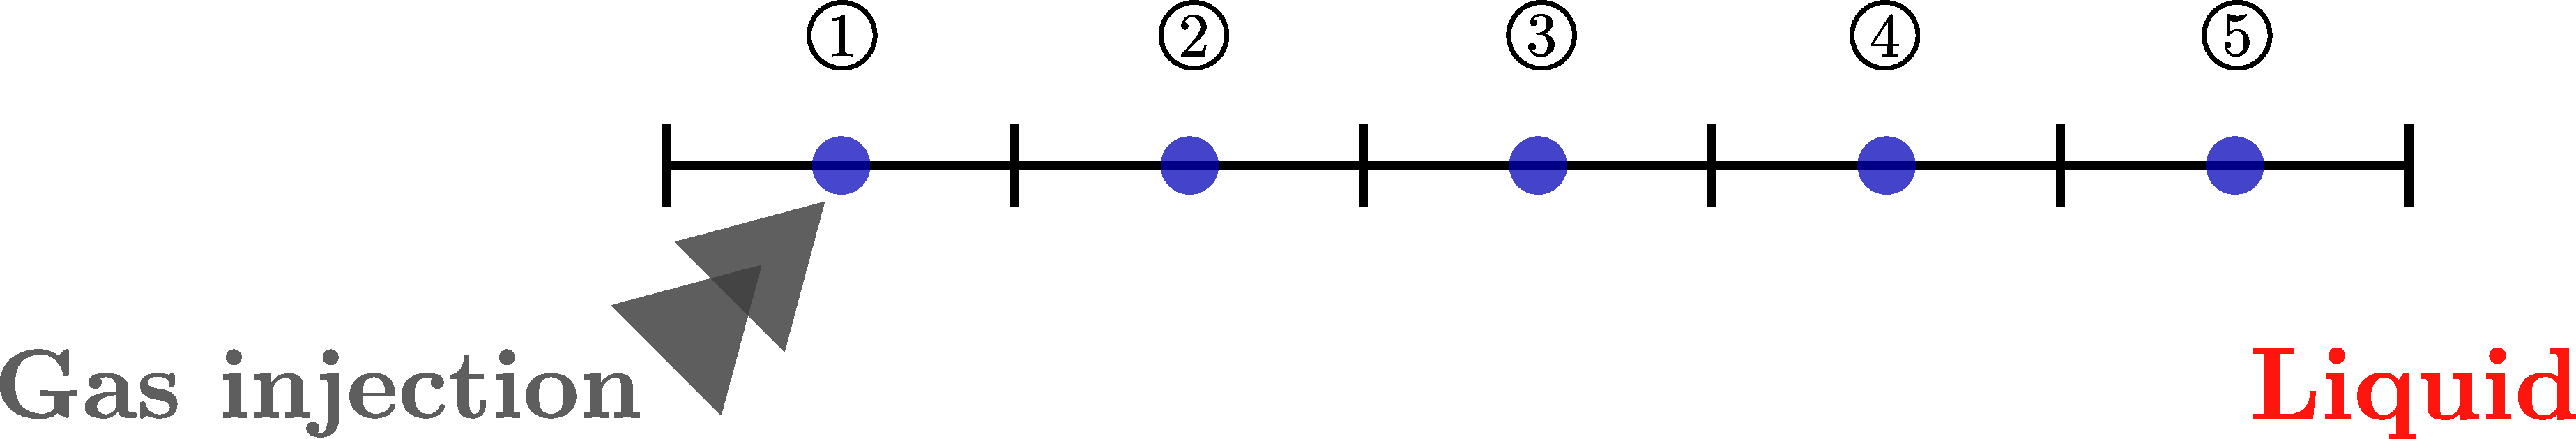
\includegraphics[width= 1 \textwidth]{fig_article_chap_3/num_exp_finite_vol}
\end{figure}

\end{frame}
% 
%% VIOLATION COMPLEMENTARITY CONSTRAINTS
% \begin{frame}
%  \frametitle{Violation of the complementarity constraints}
% \begin{figure}
% \centering
% 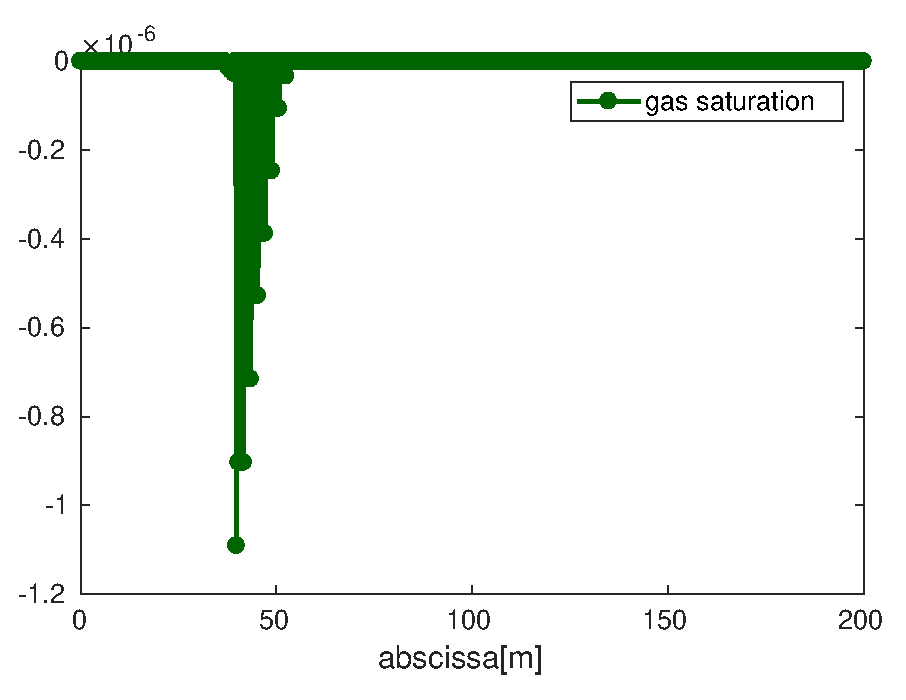
\includegraphics[width=0.45\textwidth]{fig_article_chap_3/gas_saturation_neg_gmres_iter2_newtoninter_4} \qquad
% 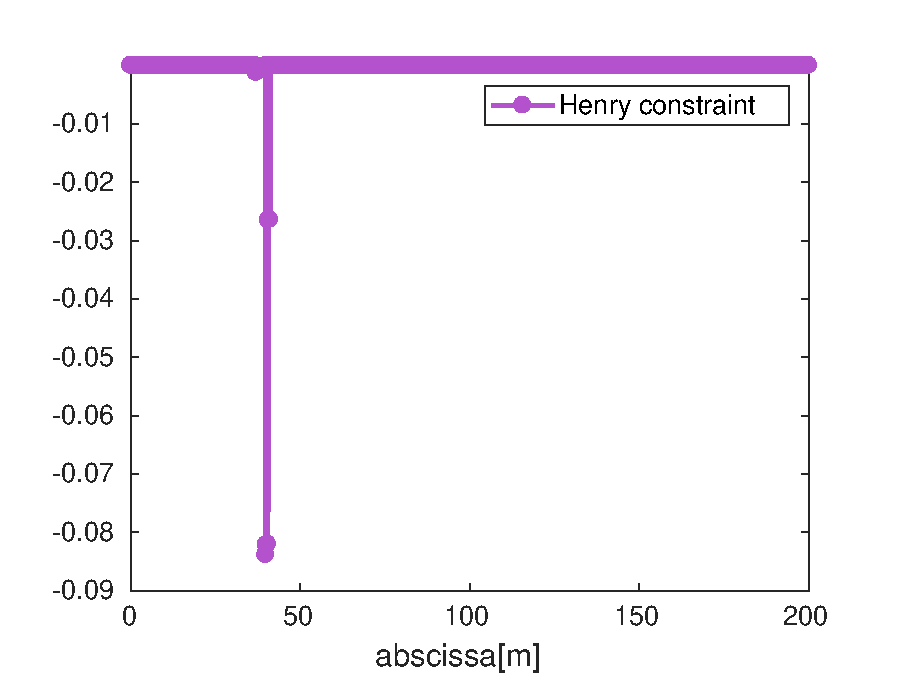
\includegraphics[width=0.48\textwidth]{fig_article_chap_3/henry_constraint_neg_gmresiter2_newton_iter4}
% \end{figure}
% \end{frame}
%
\begin{frame}
\frametitle{Phase transition estimator}

  \begin{overprint}
    \onslide<1> \scriptsize{\textcolor{red}{\textbf{\bm{$t=2500$} years}}} 
\begin{figure}
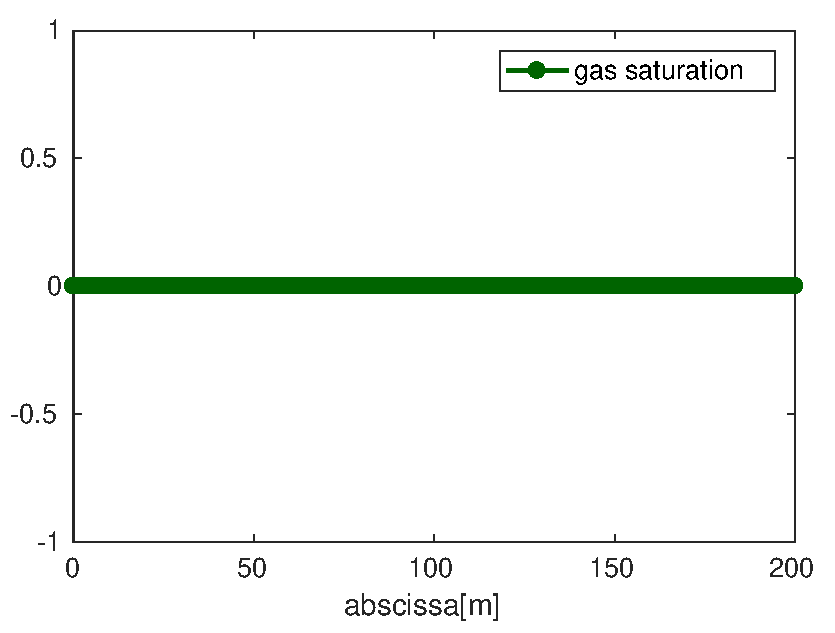
\includegraphics[width=0.47\textwidth]{fig_article_chap_3/satur_gas_init_time2}
\quad
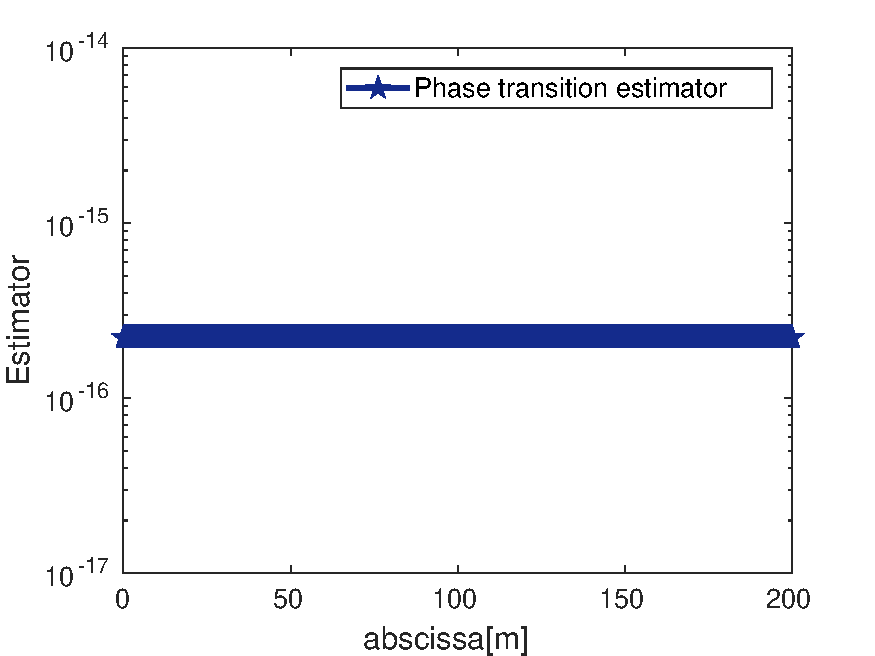
\includegraphics[width=0.47\textwidth]{fig_article_chap_3/MODIF_phase_transition_estimator_appearance_gas_nt=inittime_cv} 
    \end{figure}
\onslide<2>
\scriptsize{\textcolor{red}{ \textbf{\bm{$t = 1.25 \times 10^4$} years}}}
\begin{figure}
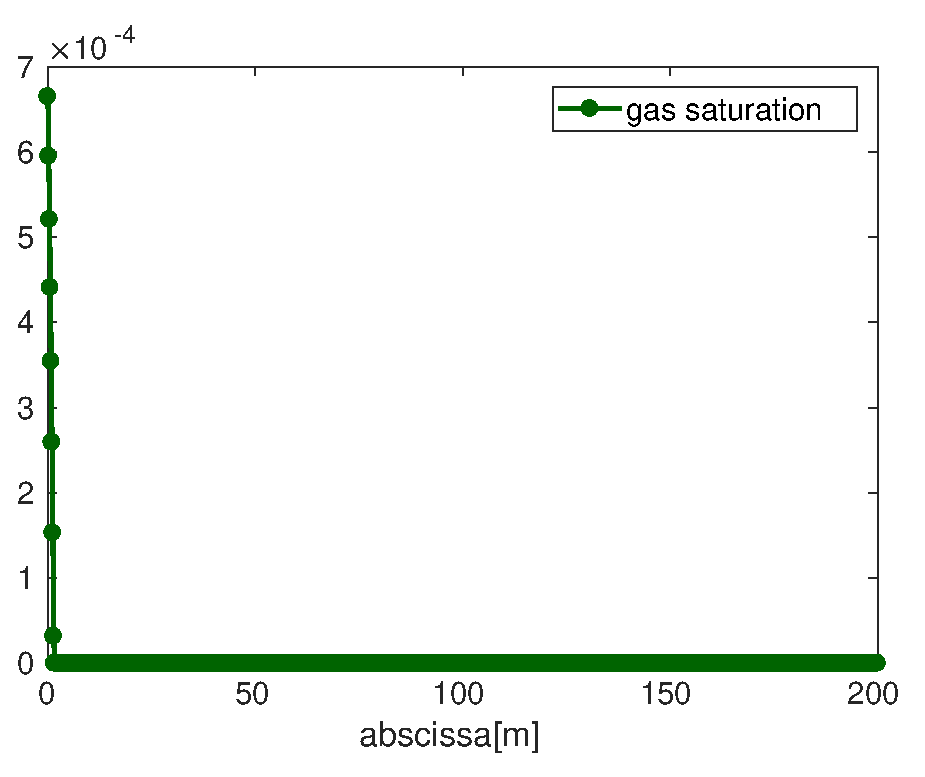
\includegraphics[width=0.45\textwidth]{fig_article_chap_3/satur_gas_appearance.eps}
 \quad
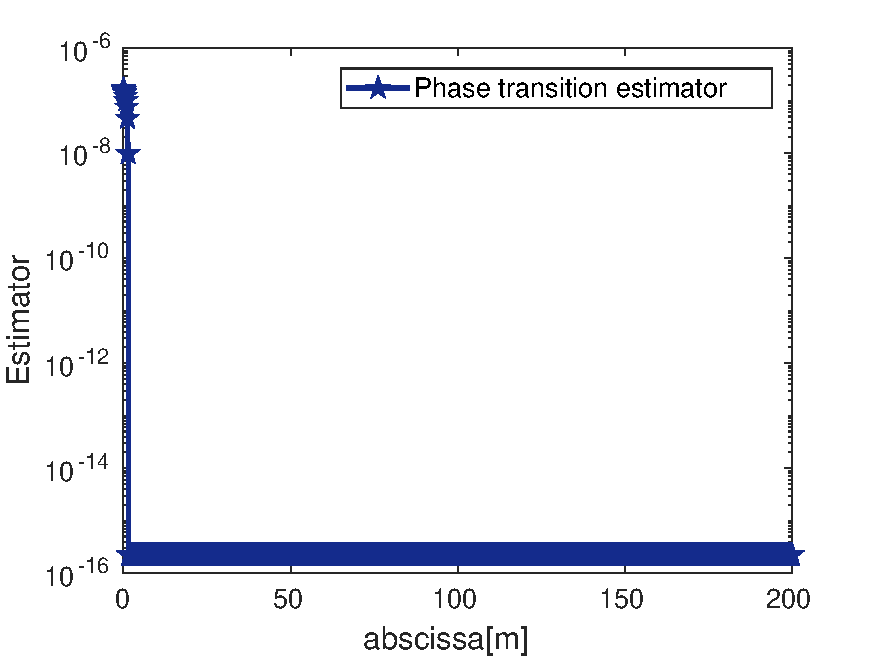
\includegraphics[width=0.47\textwidth]{fig_article_chap_3/MODIF_phase_transition_estimator_appearance_gas_nt=2_cv}
\end{figure}    

\onslide<3>
\scriptsize{ \textbf{\textcolor{red}{ \bm{$t = 4.25 \times 10^4$} years}}}
\begin{figure}
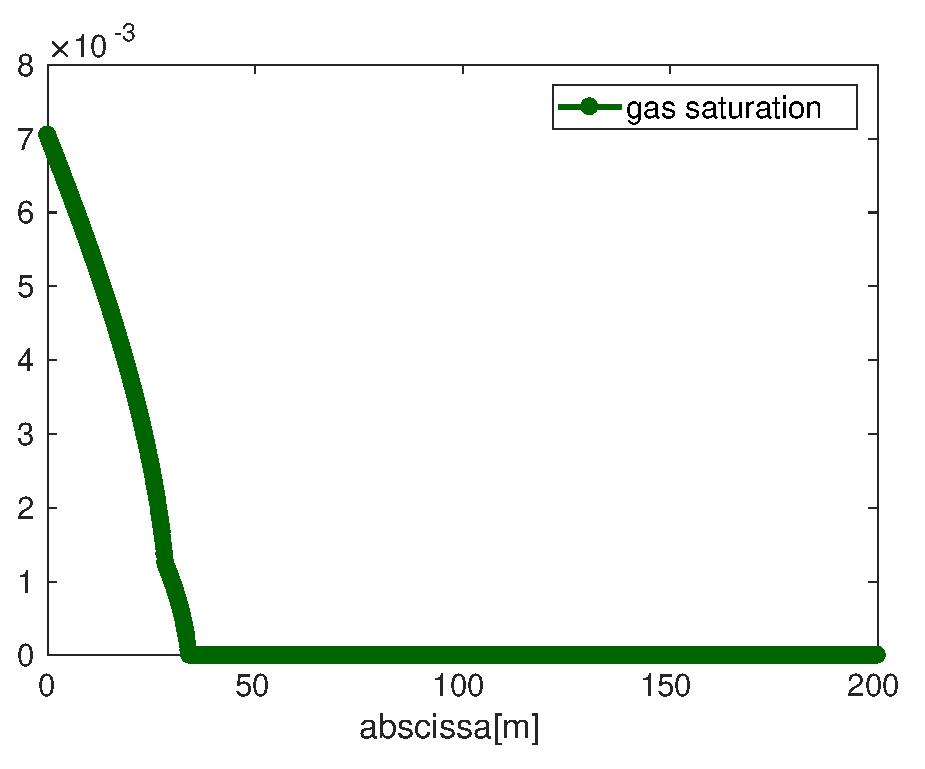
\includegraphics[width=0.45\textwidth]{fig_article_chap_3/satur_gas_after_appearance.eps}
\quad
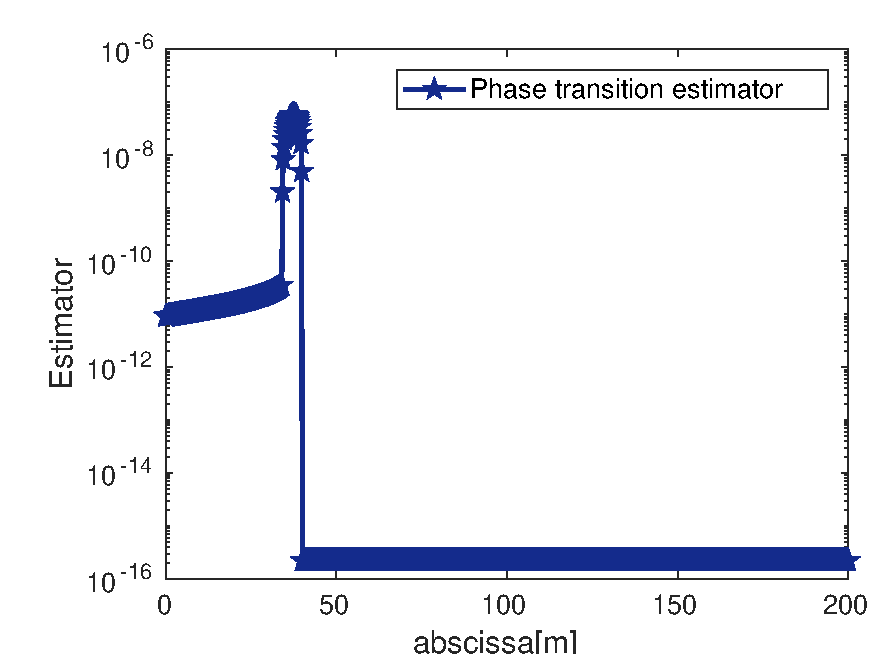
\includegraphics[width=0.47\textwidth]{fig_article_chap_3/MODIF_phase_transition_estimator_appearance_gas_nt=9_cv}
\end{figure}
\end{overprint}
 \end{frame}
%
\begin{frame}
\frametitle{Overall performance $\gammalin = \gammaalg = 10^{-3}$}
\begin{figure}
\centering
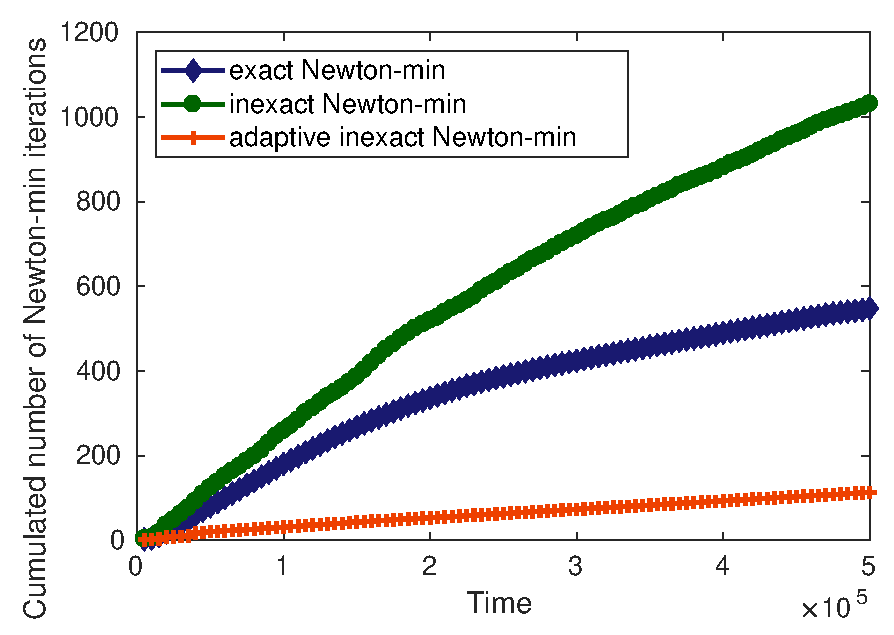
\includegraphics[width=0.47\textwidth]{fig_article_chap_3/Cumulated_number_Newton_iterations_three_methods_Nx_1000}
\hspace{0.6 cm}
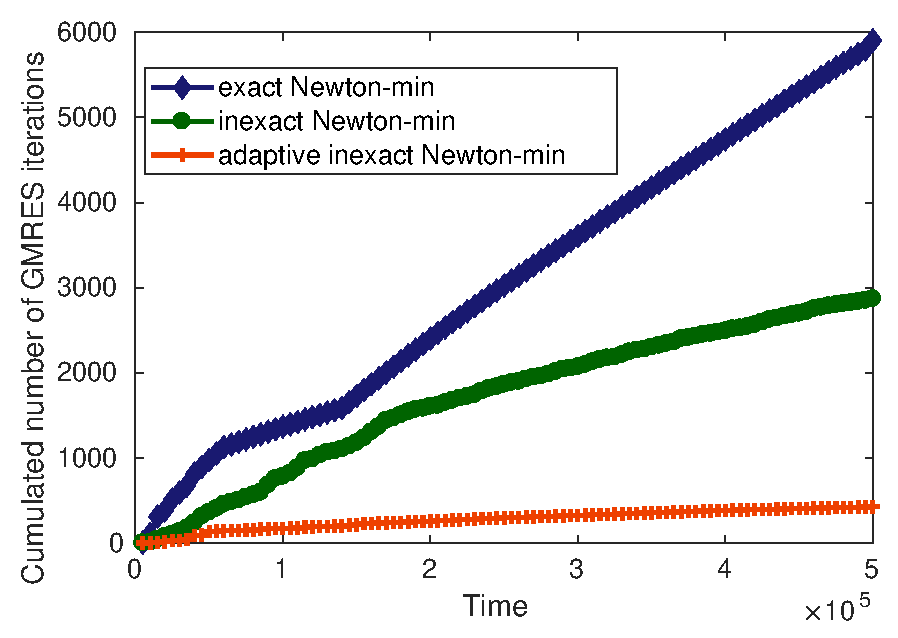
\includegraphics[width=0.47\textwidth]{fig_article_chap_3/Cumulated_number_gmres_iterations_three_methods_Nx_1000}
\end{figure}
\end{frame}
%
\begin{frame}
\frametitle{Accuracy $\gammalin = \gammaalg = 10^{-3}$}
\vspace{-0.1 cm}
\textcolor{cadmiumgreen}{\hspace{2 cm} $t = 1.05 \times 10^5$ years \hspace{5 cm} $t = 3.5 \times 10^5$ years}
\begin{figure}
\centering
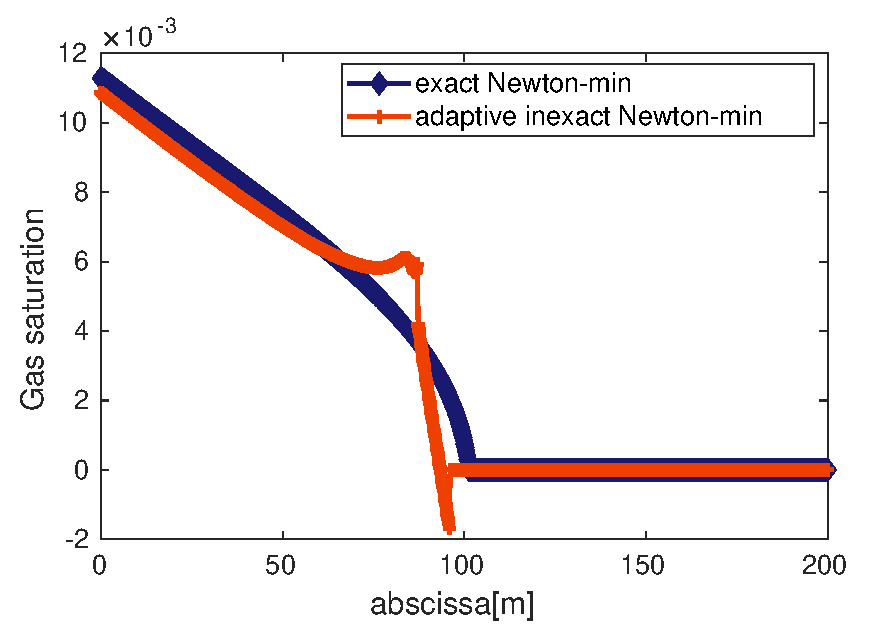
\includegraphics[width=0.48 \textwidth]{fig_article_chap_3/comparaison_plot_gas_saturations_exact_adapt_inexact_gamma_lin_gamma_alg_10-3_nt_21}
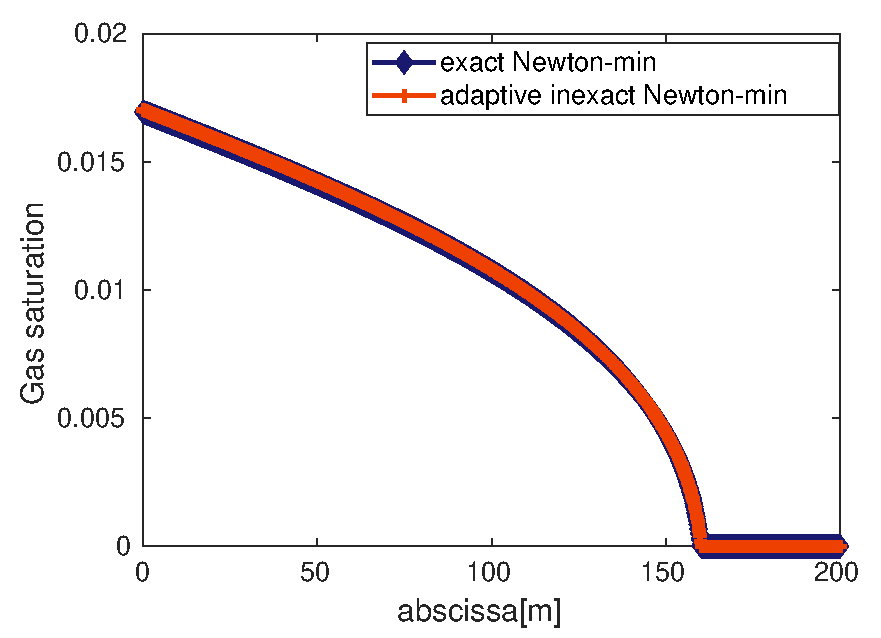
\includegraphics[width=0.48 \textwidth]{fig_article_chap_3/comparaison_plot_gas_saturations_exact_adapt_inexact_gamma_lin_gamma_alg_10-3_nt_70}
\end{figure}
\end{frame}
%
%% COMPLEMENTS NFB
% \begin{frame}
% \frametitle{Complements: Newton--Fischer--Burmeister}
% \vspace{-0.3 cm}
% \textcolor{cadmiumgreen}{
% \begin{equation*}
% \left[\fFB (\ba, \bb)\right]_l = \sqrt{\ba_l^2 + \bb_l^2} - (\ba_l + \bb_l) \quad l=1,\ldots,\Nsp.
% \end{equation*}
% }
% {\begin{table}
% \centering
% \begin{tabular}{lll}
% \hline\noalign{\smallskip}
% $\left(\gammaalg,\gammalin\right)$ & \hspace{-0.3 cm} \parbox{6.5 cm}{Cumulated number of Newton--Fischer--Burmeister iterations} &   \parbox{5 cm}{Cumulated number of GMRES  iterations}  \\
% \noalign{\smallskip}\hline\noalign{\smallskip}
% $\left(10^{-1},10^{-1} \right)$ & \qquad 100 & \quad \qquad 428 \\
% $\left(10^{-3},10^{-3}\right)$ & \qquad 119 & \quad \qquad 751 \\
% $\left(10^{-3},10^{-6}\right)$ & \qquad 482 & \quad \qquad 2074 \\
% $\left(10^{-6},10^{-3}\right)$ & \qquad 117 & \quad \qquad 1694 \\
% \textcolor{blue}{\textbf{Exact resolution}} & \qquad \textcolor{blue}{\textbf{757}} & \quad \hspace{0.2 cm} \quad \textcolor{blue}{\textbf{10089}} \\
% \noalign{\smallskip}\hline
% \end{tabular}
% \end{table}
% }

% \invisible<1>{
% \textcolor{red}{\textbf{Adaptive inexact resolution is faster than exact resolution. It saves roughly $90 \%$  of the iterations.}}
% \\
% \invisible<2>{
% \textcolor{red}{\textbf{Adaptive Newton-min is faster than Adaptive Newton--Fischer--Burmeister. It saves roughly $40 \%$ of the iterations.}}
% \invisible<3>{
% }}}
% \end{frame}
%
%
